\documentclass[11pt,a4paper]{article}
\usepackage[a4paper, total={7in, 10.25in}]{geometry}


\usepackage{color}
\usepackage{graphicx}
\usepackage{wrapfig}
\usepackage{fancyhdr}
\usepackage{tocloft}
\usepackage{multicol}
\usepackage{hyperref}
\usepackage{tabularx}
\usepackage{array}
\usepackage[export]{adjustbox}
\usepackage{listings}
\usepackage{xcolor}
\usepackage{amsmath}

    \definecolor{codegreen}{rgb}{0,0.6,0}
    \definecolor{codegray}{rgb}{0.5,0.5,0.5}
    \definecolor{codepurple}{rgb}{0.58,0,0.82}
    \definecolor{backcolour}{rgb}{1,1,1}

    \lstdefinestyle{mystyle}{
        backgroundcolor=\color{backcolour},   
        commentstyle=\color{codegreen},
        keywordstyle=\color{magenta},
        numberstyle=\tiny\color{codegray},
        stringstyle=\color{codepurple},
        basicstyle=\ttfamily\footnotesize,
        breakatwhitespace=false,         
        breaklines=true,                 
        captionpos=b,                    
        keepspaces=false,                 
        numbers=left,                    
        numbersep=5pt,                  
        showspaces=false,                
        showstringspaces=false,
        showtabs=false,                  
        tabsize=2
    }



\renewcommand{\cftsecleader}{\cftdotfill{\cftdotsep}}
\graphicspath{ {./images/} }
\hypersetup{
    colorlinks=true,
    linkcolor=blue,
    citecolor=black,
    filecolor=magenta,      
    urlcolor=cyan,
    pdftitle={Overleaf Example},
    pdfpagemode=FullScreen,
    }
\pagestyle{fancy}
\setlength{\headheight}{18pt}
\fancyhead[L]{\textit{EN3150 Pattern Recognition : Assignment 02}}
\fancyfoot[L]{\textit{Department of Electronic and Telecommunication \\University of Moratuwa}}

\title{DEPARTMENT OF ELECTRONIC AND TELECOMMUNICATION
UNIVERSITY OF MORATUWA

\vspace{10pt}

{\large{\textsc{EN 3150: Pattern recognition}}}

{\textsf{This is offered as a "EN 3150: Pattern Recognition" module's partial completion.}}

\vspace{30pt}

\includegraphics[scale=1.20]{images/University_of_Moratuwa_logo.png}

{\textsf{\textbf{Assignment 02 : Kernel methods}}}}


\author{200686J : Vishagar A.}

\date{$2^{nd}$ of November, 2023}

\begin{document}

\maketitle

\newpage

\begin{abstract}
    \textit{This report deals with the explanation of the solutions for the given questions in the assignment 02 of the EN3150 module. The solutions are explained in a way that it is easy to understand and follow. The solutions are explained with the help of the code snippets and the results.We are mainly focussed on using the kernel methods and utilizing it for Support vector machine algorithm in the case of non seperable data.}    
\end{abstract}    

\vspace{50pt}
\tableofcontents


\newpage

\twocolumn

\section{Kernel Methods}
\subsection{Question 01}

\begin{equation}
    \phi{(x)} =  (x,\sqrt{2}x,x^2)
\end{equation}

for one dimensional data,

\begin{equation}
    \phi{(z)} =  (z,\sqrt{2}z,z^2)
\end{equation}

\begin{equation}
    \phi{(z)}*\phi{(x)} =  (1 + 2xz + x^2z^2)
\end{equation}

\begin{equation}
    K(x,z) =  (1 + 2xz + x^2z^2)
\end{equation}

\begin{equation}
    K(x,z) =  (1 + xz)^2   
\end{equation}

\subsection{Question 02}

\begin{equation}
    K(x,z) =  (1 + xz)^2   
\end{equation}

for 2 dimensional input data,

\begin{equation}
    K(x,z) =  (1 + x_1z_1 + x_2z_2)^2   
\end{equation}

\subsection{Question 03}

Finding the mapping function for the given kernel function,

\begin{equation}
    K(x,z) =  (1 + x_1z_1 + x_2z_2)^2 
\end{equation}

\begin{equation}
    K(x,z) =  (1 + x_1z_1 + x_2z_2)(1 + x_1z_1 + x_2z_2)
\end{equation}

\begin{align}
    K(x,z) &=  (1 + (x_1z_1)^2 + (x_2z_2)^2 \nonumber \\
    &\quad + 2x_1z_1 + 2x_2z_2 + 2x_1z_1x_2z_2)
\end{align}

continue..


\subsection{Question 04}


\begin{equation}
    G = 
    \begin{bmatrix}
        k(x_1,x_1) & k(x_1,x_2) & k(x_1,x_3) & k(x_1,x_4) \\
        k(x_2,x_1) & k(x_2,x_2) & k(x_2,x_3) & k(x_2,x_4) \\
        k(x_3,x_1) & k(x_3,x_2) & k(x_3,x_3) & k(x_3,x_4) \\
        k(x_4,x_1) & k(x_4,x_2) & k(x_4,x_3) & k(x_4,x_4) 
    \end{bmatrix}
\end{equation}

\begin{equation}
    G = 
    \begin{bmatrix}
        27 & 24 & 15 & 71 \\
        24 & 26 & 21 & 79 \\
        15 & 21 & 21 & 65 \\
        71 & 79 & 65 & 245
    \end{bmatrix}
\end{equation}


\newpage

List of eigen values,
\begin{equation}
    \lambda_1 = 315.858
\end{equation}

\begin{equation}
    \lambda_2 = 9.2378
\end{equation}

\begin{equation}
    \lambda_3 = 2.8946
\end{equation}

\begin{equation}
    \lambda_4 = 0.0096
\end{equation}

All eigen values are \textbf{non-negative} as well as the matrix is a \textbf{symmetric matrix}. Therefore the matrix is \textbf{positive semi definite matrix}. And also this will be a valid kernel.

\section{Implementation of Kernel and Results}

\subsection{Data Generation and Visualization}

\lstset{style=mystyle}
\lstinputlisting[language=Octave]{code1.py}

{\begin{figure}[h]
    \centering
    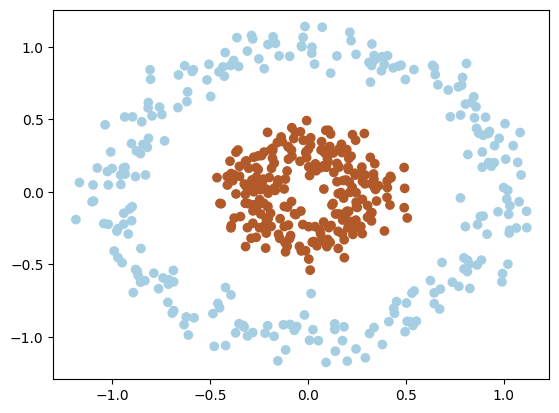
\includegraphics[width=1.0\linewidth]{images/1.png}
    \caption{Data Generation}
\end{figure}}

\newpage
\subsection{Using mapping functions}

\textbf{\textit{Funtion 01}}

\begin{equation}
    \phi : x = (x_1,x_2) \rightarrow \phi{(x)} =  (x_1,x_2,x_1^2+x_2^2)
\end{equation}

The following code was used to implement the above mentioned function.

\lstset{style=mystyle}
\lstinputlisting[language=Octave]{code2.py}
    
    {\begin{figure}[h]
        \centering
        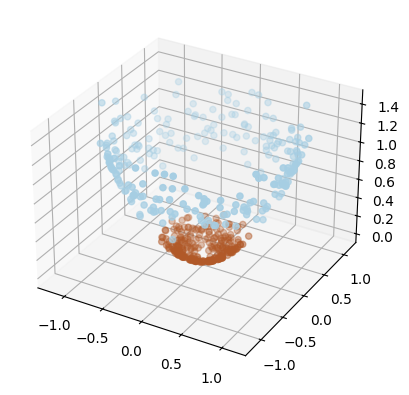
\includegraphics[width=1.0\linewidth]{images/2.png}
        \caption{Data Generation}
    \end{figure}}

We have created a data set with a factor of 0.3 and we have used the above mentioned function to map the data into a higher dimensional space.\\

From this Visualization we can see that the data is linearly seperable. We have mapped the data into a higher dimensional space and we can seed this data for our linear support vector machine algorithm.

\newpage

If we try to \textbf{increase the factor from 0.3 to 0.5,}

{\begin{figure}[h]
    \centering
    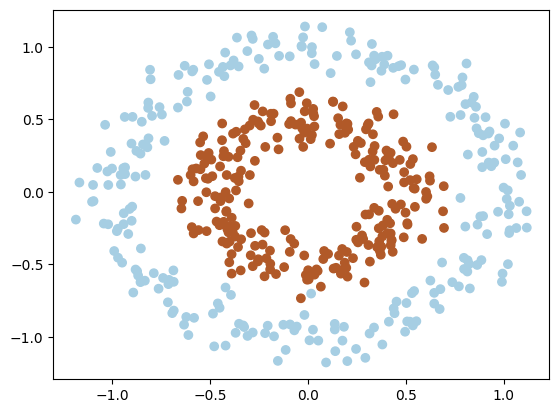
\includegraphics[width=1.0\linewidth]{images/6.png}
    \caption{Data Generation}
\end{figure}}

{\begin{figure}[h]
    \centering
    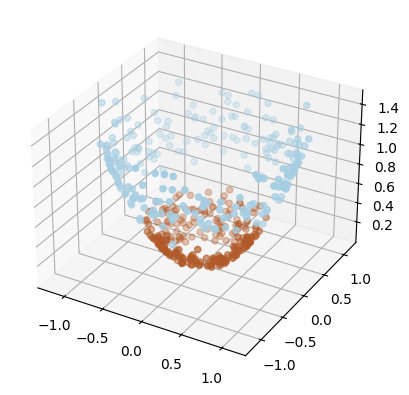
\includegraphics[width=1.0\linewidth]{images/7.png}
    \caption{Data Generation}
\end{figure}}

Normally factor determines the radius of the inner circle with respect to the radius of the out put circle.In this scenario where we increased the factor from 0.3 to 0.5 we can clearly see that the data tends to mix up, even in the higher dimensional space, the data from the two classes tends to mix up.\\\\


\textbf{\textit{Funtion 02}}\\

Now for the same data (factor = 0.3) if we use the following mapping function,

\begin{equation}
    \phi : x = (x_1,x_2) \rightarrow \phi{(x)} =  (x_1^2,x_2^2,x_1x_2)
\end{equation}

\newpage

And the following code was used to implement the above mentioned function.

\lstset{style=mystyle}
\lstinputlisting[language=Octave]{code3.py}


{\begin{figure}[h]
    \centering
    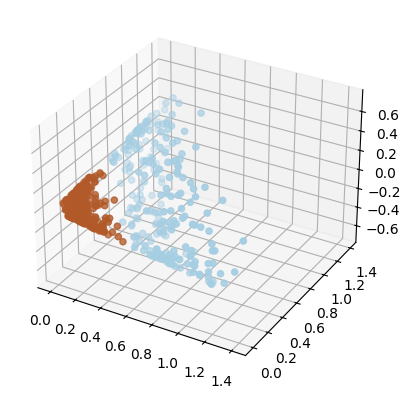
\includegraphics[width=1.0\linewidth]{images/3.png}
    \caption{Data Generation}
\end{figure}}

Comparing to the above mapping this mapping seems to be somewhat better as we can clearly two clusters of data in the higher dimensional space which will be easy while seperation using a linear boudary surface. What happen here is as we are squaring the $x_{1}$ and $x_{2}$ features because of the non linear mapping and the feature expansion we can get a clear seperable data which can be distinguished by a linear decision boundary.\\\\

\newpage

\subsection{Running Linear SVC}

\textbf{\textit{For data without mapping}}\\

\lstset{style=mystyle}
\lstinputlisting[language=Octave]{code4.py}

and following were the results,

\begin{itemize}
    \item Accuracy: 
    \item Precision:  
    \item Recall: 
    \item F1 Score: 
\end{itemize}


\textbf{\textit{For data with first mapping}}\\

\lstset{style=mystyle}
\lstinputlisting[language=Octave]{code5.py}

and following were the results,

{\begin{figure}[h]
    \centering
    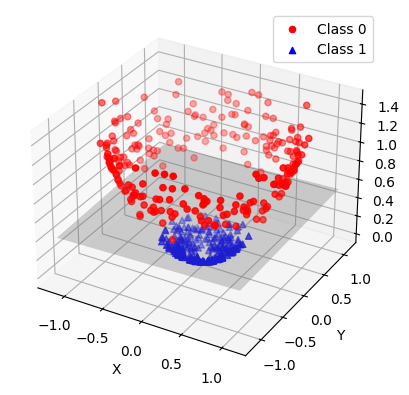
\includegraphics[width=1.0\linewidth]{images/4.png}
    \caption{Data Generation}
\end{figure}}


\begin{itemize}
    \item Accuracy: 1.0
    \item Precision: 1.0 
    \item Recall: 1.0 
    \item F1 Score: 1.0
\end{itemize}



\textbf{\textit{For data with second mapping}}\\

\lstset{style=mystyle}
\lstinputlisting[language=Octave]{code5.py}

and following were the results,

{\begin{figure}[h]
    \centering
    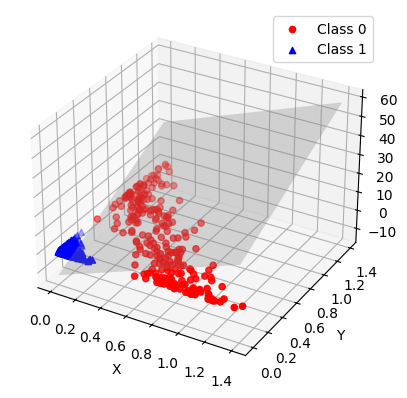
\includegraphics[width=1.0\linewidth]{images/5.png}
    \caption{Data Generation}
\end{figure}}


\begin{itemize}
    \item Accuracy: 1.0 
    \item Precision: 1.0 
    \item Recall: 1.0 
    \item F1 Score: 1.0
\end{itemize}




\section{References}

\begin{itemize}
    \item \href{https://scikit-learn.org/stable/modules/generated/sklearn.linear_model.LinearRegression.html}{Sci-kit Learn Documentation on Logistic regression}
    \item \href{https://scikit-learn.org/stable/auto_examples/compose/plot_digits_pipe.html}{Pipelining}
    \item \href{https://scikit-learn.org/stable/modules/generated/sklearn.model_selection.GridSearchCV.html}{Grid Search}
    % \item \href{ }{Github/EN3160_Assignment_01}
   
\end{itemize}

\section{Github Repository}

Following is the link to my Github repository for this assignment.\\

\href{https://github.com/Vgr20/EN3150_Assignment_04.git}{Github/EN3150\_Assignment\_04}


\end{document}




%%%%%%%%%%%%%%%%%%%%%%%%%%%%%%%%%%%%%%%%%%%%%%%%%%%%%%%%%%%%%%%%%%%%%%%%%%%%%%%%%%%%%%%%%%%%%%%%%%%%%%%%%%%%%%%%%%%%%%%%%%%%%%%%%%%%%%%%%%%%%%%%%%%%%%%%%%%%%%%%%%%%%%%%%%

% {\begin{center}
% \begin{tabular}{ | m{1.85cm} | m{0.85cm}| m{0.85cm} | m{0.85cm} | m{0.85cm} | m{0.85cm} | } 
%  \hline
%  Objectives& Weight & Design 01 & Design 02 & Design 03 & Design 04 \\  
%  \hline\hline
%  Efficiency & 10 & 7 & 8 & 8 & 9 \\
%  \hline
%  Mobility & 10 & 7 & 9 & 8 & 8 \\
%  \hline
%  Easy Maintenance & 10 & 7 & 6 & 5 & 8 \\
%  \hline
%  Refilling accessibility & 5 & 3 & 3 & 2 & 4 \\
%  \hline
%  Durability & 5 & 2 & 3 & 3 & 2 \\
%  \hline
%  Manufacture cost & 5 & 3 & 3 & 2 & 3 \\
%  \hline
%  Overall Look & 5 & 2 & 3 & 5 & 2 \\
%  \hline
%  \hline
%  Total & 50 & 31 & 35 & 33 & 36 \\
%  \hline
 
% \end{tabular}
% \end{center}}

%%%%%%%%%%%%%%%%%%%%%%%%%%%%%%%%%%%%%%%%%%%%%%%%%%%%%%%%%%%%%%%%%%%%%%%%%%%%%%%%%%%%%%%%%%%%%%%%%%%%%%%%%%%%%%%%%%%%%%%%%%%%%%%%%%%%%%%%%%%%%%%%%%%%%%%%%%%%%%%%%%%%%%%%%%


% \begin{center}
% \begin{tabular}{ | m{2cm} | m{5cm}| m{2cm} | m{6cm} | } 

%  \hline
%  Part Name & Description & Supplier & Part Link\\  
%  \hline\hline
%  NE555P & 8-pin Precise timer & Texas Instruments & \href{https://www.lcsc.com/product-detail/Timers-Clock-Oscillators_Texas-Instruments-NE555P_C46749.html}{NE555p data sheet}\\
%  \hline
%  2N2222A & Generic npn transistor & Slkor & \href{https://www.lcsc.com/product-detail/Bipolar-Transistors-BJT_Slkor-SLKORMICRO-Elec-2N2222A_C5330385.html}{2N2222A data sheet}\\
%  \hline
%   LM7805 & Linear voltage Regulators & LRC & \href{https://www.lcsc.com/product-detail/Linear-Voltage-Regulators-LDO_LRC-LR7805_C2846986.html}{Lm7805 Data sheet}\\
%  \hline
%   HC sr501 & Passive IR sensor & HC & \href{https://www.lcsc.com/product-detail/Timers-Clock-Oscillators_Texas-Instruments-NE555P_C46749.html}{HC sr501 data sheet}\\
%  \hline
%   KNSCHA ZE11000UF & 1000uF Capacitor & KNSCHA & \href{https://www.lcsc.com/product-detail/Solid-Capacitors_KNSCHA-ZE11000UF35V119EC0014_C2992586.html}{Capacitor data sheet}\\
%  \hline
%   Resistors & Resistors with different values & Texas Instruments & \href{https://www.lcsc.com/search?q=resistors%20through%20hole}{Through hole resistors}\\
%  \hline
 
% \end{tabular}  
% \end{center}
%%%%%%%%%%%%%%%%%%%%%%%%%%%%%%%%%%%%%%%%%%%%%%%%%%%%%%%%%%%%%%%%%%%%%%%%%%%%%%%%%%%%%%%%%%%%%%%%%%%%%%%%%%%%%%%%%%%%%%%%%%%%%%%%%%%%%%%%%%%%%%%%%%%%%%%%%%%%%%%%%%%%%%%%%%